\PassOptionsToPackage{usenames,dvipsnames}{xcolor}
\documentclass[use boldface]{beaulivre}
\usepackage{mmcesim-doc}

\newcommand{\mmCEsimVersion}{0.2.2}

\begin{document}

\frontmatter

\TitlePage [
    color = { main = TitleMainColor, back = TitleBackColor!60!white },
    logo = {\includegraphics[width=2.2cm]{img/logo/mmCEsim_logo_256.png}
      \raisebox{8mm}{\scalebox{1.3}{\rlap{\begin{tabular}{c}
        \fontsize{23}{30}\selectfont\sffamily\bfseries\textcolor{TitleMainColor}{mmCEsim} \\
        {\hypersetup{urlcolor=black}\url{https://mmcesim.org}}
      \end{tabular}}}}
    }
  ]
  {
    , title     = mmCEsim Documentation \& Tutorials
    , subtitle  = {
                    \textsc{Task-oriented mmWave Channel Estimation Simulation}\\[10pt]
                    \normalsize Version \texttt{\mmCEsimVersion}
                  }
    , author    = Wuqiong Zhao (Teddy van Jerry)
    , date      = {\today{}}
    , license   = {% counter the \vfill in ProjLib
\vspace*{-\fill}

\noindent
The application `mmCEsim' and this document
(\textsc{mmCEsim Documentation \& Tutorials})
are open source and distributed by an MIT License.
\newline

\noindent
MIT License
\newline

\noindent
Copyright \copyright~2022 -- 2023 Wuqiong Zhao (Teddy van Jerry)
\newline

\noindent
Permission is hereby granted, free of charge, to any person obtaining a copy
of this software and associated documentation files (the ``Software''), to deal
in the Software without restriction, including without limitation the rights
to use, copy, modify, merge, publish, distribute, sublicense, and/or sell
copies of the Software, and to permit persons to whom the Software is
furnished to do so, subject to the following conditions:
\newline

\noindent
The above copyright notice and this permission notice shall be included in all
copies or substantial portions of the Software.
\newline

\noindent
THE SOFTWARE IS PROVIDED ``AS IS'', WITHOUT WARRANTY OF ANY KIND, EXPRESS OR
IMPLIED, INCLUDING BUT NOT LIMITED TO THE WARRANTIES OF MERCHANTABILITY,
FITNESS FOR A PARTICULAR PURPOSE AND NONINFRINGEMENT. IN NO EVENT SHALL THE
AUTHORS OR COPYRIGHT HOLDERS BE LIABLE FOR ANY CLAIM, DAMAGES OR OTHER
LIABILITY, WHETHER IN AN ACTION OF CONTRACT, TORT OR OTHERWISE, ARISING FROM,
OUT OF OR IN CONNECTION WITH THE SOFTWARE OR THE USE OR OTHER DEALINGS IN THE
SOFTWARE.
\newline
\newline

\noindent
The latest edition of this document (\textsc{mmCEsim Documentation \& Tutorials})
can be freely accessed online at \url{https://pub.mmcesim.org/mmCEsim-doc.pdf}
or \href{https://mmces.im/pdf}{\texttt{mmces.im/pdf}} for short.
\newline

\noindent
Edition \mmCEsimDate{}
(corresponding to mmCEsim version \mmCEsimVersion).

\vfill
\noindent
mmCEsim Website: \url{https://mmcesim.org}

\noindent
Source of This Document: \url{https://github.com/mmcesim/mmcesim-doc}
}
  }

\begingroup
\turnoffhypercolor
\tableofcontents
\endgroup

\chapter{Preface}
\begin{tip}
  mmCEsim documentation \& tutorials are updating from v0.2.0 to v0.3.0!
\end{tip}

As a researcher in wireless communications and signal processing,
I have always had a passion for programming.
Since my first year at university
when I started using C++ to accomplish amazing tasks,
I have been convinced of the importance of software in research.

Despite this, many researchers underestimate the significance of software
in implementation, simulation, and verification of algorithms.
Scientific software and programming languages, along with libraries,
have been the driving force behind advances in science.
Therefore, I am proud to present mmCEsim,
an open-source software that is not only easy to use but also free for all.

The idea for mmCEsim originated from the tedious process of writing C++ code
for implementing compressed channel estimation for
reconfigurable intelligent surface (RIS)-assisted multiple-input multiple-output (MIMO) systems.
I was driven by a desire to get rid of these repetitive tasks and eliminate the need
to spend so much time setting up simulations.
Inspired by NYUSIM, I decided to create my own simulation software.

To make it even easier to use, I designed a programming language called ALG,
with simple syntax for describing algorithms.
This language can be converted into other languages, such as C++ and \textsc{Matlab}, for simulation.
To use mmCEsim, simply configure your system settings, decide on your channel estimation algorithm,
and extend the sounding and estimation process with ALG.

At present, mmCEsim supports channel estimation based on compressed sensing in mmWave
and is expected to be more general in the future.
It is still under active development and evolving.

I would like to thank my professor, seniors, and fellow students for their help and inspiration.
I would also like to express my gratitude to Jinwen Xu for designing the elegant \LaTeX{} template,
\texttt{beaulivre}, which has made this document possible.

\begin{flushright}
  \textsc{Wuqiong Zhao}

  Nanjing, China

  \TheDate{\the\year/\the\month}[only-year-month]
\end{flushright}


\begingroup
\turnoffhypercolor
\cleardoublepage
\phantomsection
\addcontentsline{toc}{chapter}{List of Figures}
\listoffigures

\cleardoublepage
\phantomsection
\addcontentsline{toc}{chapter}{List of Tables}
\listoftables

\endgroup

\mainmatter

\part{Preliminary}
\parttext{Make preparations before we start.}

\chapter{Preview}
Before diving into documentation details, let's first have a preview of mmCEsim.
Maybe you are not sure whether your research or study need this powerful tool,
then read this chapter to have a glimpse of mmCEsim.

\section{Introduction}

The application is dedicated to simulate
millimeter wave (mmWave) channel estimation:
\[
  \text{mmCEsim}
  =\text{\textbf{mm}Wave}
  +\text{\textbf{C}hannel \textbf{E}stimation}
  +\text{\textbf{sim}ulation},
\]
where reconfigurable intelligent surface (RIS),
also known as intelligent reflecting surface (IRS) \cite{wu2019towards} is supported
for multiple input multiple output (MIMO) systems.

\begin{figure}[htbp]
  \includegraphics[width=\linewidth]{img/badge/mmCEsim_badge.png}
  \caption{mmCEsim banner.}
\end{figure}

We offer a task-oriented simulation software for researchers to focus on algorithms only
without being bothered by coding.

\section{Features}

Here is a list of basic features of mmCEsim:
\begin{itemize}
  \item Task-oriented mmWave channel estimation formulation;
  \item Customizable system model;
  \item Extendable algorithms with our designed ALG language;
  \item Multiple RISs support;
  \item Automatic report generation (in plain text and \LaTeX{} PDF);
  \item Well-written documentation with examples and tutorials.
\end{itemize}

\section{Algorithm Background}

The task-oriented channel estimation for (RIS-assisted) mmWave MIMO systems
is implemented with compressed sensing (CS),
which exploits the sparsity of mmWave channels.

\section{Software Implementation}
Based on the algorithm background,
we implement this software with
command line interface (CLI),
graphic user interface (GUI),
web application and a VS Code extension.
The workflow\index{workflow} of mmCEsim is depicted in Fig.~\ref{fig:mmCEsim_workflow}.

\begin{figure}[htbp]
  \centering\sffamily
  \begin{tikzpicture}[
    , thick
    , node distance = 5mm and 8mm
    , n/.style = {
      , draw
      , fill = #1!20
      , minimum height = 8mm
      , minimum width = 22mm
      , align = center
    }
    , null n/.style = {
      , inner sep = 0
      , outer sep = 0
    }
  ]
    \node (gui) [n = mypurple] {GUI App};
    \node (config) [below = 8mm of gui, n = myblued, font = \small] {Configuration\\File (YAML)};
    \node (alg) [below = 4mm of config, n = myblued, font = \small] {Algorithm\\Library (ALG)};
    \node (export) [right, xshift = 10mm, n = mygreen, font = \large] at ($(config.south east)!.5!(alg.north east)$) {Code\\Exporter};
    \node (py) [n = myyellow, right = 9mm of export, minimum height = 5mm, minimum width = 25mm, font = \small] {Python (NumPy)};
    \node (cpp) [n = myyellow, above = 1mm of py, minimum height = 5mm, minimum width = 25mm, font = \small] {C++ (Armadillo)};
    \node (m) [n = myyellow, below = 1mm of py, minimum height = 5mm, minimum width = 25mm, font = \small] {\textsc{Matlab}/Octave};
    \node (code) [above = .5mm of cpp] {Exported Code};
    \node (run) [n = mygreen, right = 9mm of py, font = \large] {Code\\Runner};
    \node (rpt) [n = mygreen, right = of run, font = \large] {Report\\Generator};
    \draw [-Latex] (run) -- (rpt);
    \draw [-Latex, gray] (gui) -- (config);
    \foreach \x in {config, alg} {
      \draw (\x.east) -| ([xshift = -5mm]export.west);
    }
    \draw [Latex-] (export.west) -- ++ (-5mm, 0);
    \draw [-Latex] (export.east) -- ++ (8mm, 0);
    \draw [Latex-] (run.west) -- ++ (-8mm, 0);
    \node [fit = (code)(m), inner sep = 1mm, draw, dashed, Blue] {};
    \draw [-Latex, gray, dashed] (gui) -| node [null n] (tmp-1) {} (export);
    \draw [-Latex, gray, dashed] (tmp-1) -| node [null n] (tmp-2) {} (run);
    \draw [-Latex, gray, dashed] (tmp-2) -| (rpt);
    % \begin{scope}[on background layer]
    % \end{scope}
  \end{tikzpicture}%
  \caption{mmCEsim workflow.}
  \label{fig:mmCEsim_workflow}
\end{figure}


\chapter{Installation}
\section{Download Binary}
You can download the built binary of mmCEsim from \href{https://github.com/mmcesim/mmcesim/releases}{GitHub releases}.
The built CLI binaries include support for Linux (x86), macOS (x64 and arm) and Windows (x86).

They all statically link to libraries, so theoretically no dependency is needed.

\begin{tip}[Note]
  Since GitHub Actions currently only provide x86\_64 machines,
  the binary for macOS with arm architecture is built manually on my MacBook Air with an M1 chip.
\end{tip}

\section{Build from Source}

Since mmCEsim is built with CMake, so you can easily build the source on Unix-based systems.
For Windows, I think there are similar ways.

On a Unix-based system, you can simply use the following code to build and install mmCEsim.
\begin{lstlisting}[language=sh, morekeywords={git, mkdir, cmake, make, sudo}, alsoletter={.}]
git clone https://github.com/mmcesim/mmcesim.git --recurse-submodules
cd mmcesim
mkdir build
cmake . build
cd build
make
sudo make install
\end{lstlisting}

\begin{remark}
  The option \texttt{--recurse-submodules} is required because some dependencies of mmCEsim
  are managed by Git submodules.
\end{remark}

You need to have a C++ compiler that supports C++17 standard,
and have installed the Boost library (statically) of minimum version \texttt{1.70.0} on your system.
You can install them easily on Unix-based systems with your favourite package manager.
For Windows users, please follow the official instruction of Boost.
\begin{lstlisting}[language=sh, morekeywords={sudo, apt, pacman, port, brew}]
# Debian, Ubuntu
sudo apt install libboost-dev
# Arch
sudo pacman -Ss boost
# macOS
sudo port install boost # with MacPorts
brew install boost      # with HomeBrew
\end{lstlisting}

If you want to build the GUI app as well, you need to install Qt6.
\newline

Some options can be configured when calling \texttt{cmake}.
\begin{itemize}
  \item \textcolor{forestgreen}{\texttt{CMAKE\_BUILD\_TYPE}}: Build type (default as \texttt{Release})
  \item \textcolor{forestgreen}{\texttt{CMAKE\_INSTALL\_PREFIX}}: Installation prefix (default as system path)
  \item \textcolor{forestgreen}{\texttt{MMCESIM\_BUILD\_ASTYLE}}: Build \texttt{astyle} code ormatter (default as \texttt{ON})
  \item \textcolor{forestgreen}{\texttt{MMCESIM\_BUILD\_LOG}}: Build mmCEsim log tool (default as \texttt{ON})
  \item \textcolor{forestgreen}{\texttt{MMCESIM\_BUILD\_MAINTAIN}}: Build mmCEsim maintenance tool (default as \texttt{ON})
  \item \textcolor{forestgreen}{\texttt{MMCESIM\_BUILD\_GUI}}: Build mmCEsim GUI App with Qt (default as \texttt{OFF})
  \item \textcolor{forestgreen}{\texttt{MMCESIM\_APPLE\_COPY\_SH}}: Copy additional shell script for macOS (default as \texttt{OFF}).
  \item \textcolor{forestgreen}{\texttt{MMCESIM\_TESTS}}: Run mmCEsim tests (default as \texttt{ON}).
\end{itemize}

For example, you may use \lstinline[morekeywords={cmake}]{cmake . build -D CMAKE_INSTALL_PREFIX=usr/mmcesim}
to install mmCEsim to the directory \texttt{usr/mmcesim}.

\section{Troubleshooting}
\subsection{macOS Safety Warning}
You may view a safety warning after downloading the binary from GitHub Releases.
The \texttt{trust\_mmcesim.sh} is a script to remove that warning.
(Give the script proper permission before running in its directory).
Technically, it does \lstinline[morekeywords={xattr}]{xattr -r -d com.apple.quarantine <binary>}.


\part{Documentation}
\parttext{Every syntax and option in details.}

\chapter{CLI Application}\label{d:chap:cli}
\section{CLI Options}\index{CLI command}
With \texttt{mmcesim -h}, you can view all supported commands and options.
\begin{lstlisting}
mmCEsim 0.2.0  (C) 2022-2023 Wuqiong Zhao
Millimeter Wave Channel Estimation Simulation
=============================================

Usage: ./mmcesim <command> <input> [options]

Commands:
  sim [ simulate ]       run simulation
  dbg [ debug ]          debug simulation settings
  exp [ export ]         export code
  config                 configure mmCEsim options
  (Leave empty)          generic use

Allowed options:

Generic options:
  -v [ --version ]       print version string
  -h [ --help ]          produce help message
  --gui                  open the GUI app

Configuration:
  -o [ --output ] arg    output file name
  -s [ --style ] arg     style options (C++ only, with astyle)
  -l [ --lang ] arg      export language or simulation backend
  --value arg            value for configuration option
  -f [ --force ]         force writing mode
  -V [ --verbose ]       print additional information
  --no-error-compile     do not raise error if simulation compiling fails
  --no-term-color        disable colorful terminal contents
\end{lstlisting}

The allowed commands are explained in the following.

\subsection{exp}\indexCLIcmd{exp}
Command \texttt{exp} exports the \texttt{.sim} configuration and corresponding \texttt{.alg} algorithms
to a selected language.
Currently, only export to C++ with Armadillo is supported.

\subsection{sim}\indexCLIcmd{sim}
Command sim simulates the exported code with the selected backend. Currently, only C++ with Armadillo is supported.

So far, only C++ compiler \texttt{g++} (default) and \texttt{clang++} are supported which can be configured with option \hyperref[d:subsec:config]{\texttt{config}}.
You may also need to configure additional C++ flags with \texttt{config cppflags} if by default the compiler cannot find
\href{https://arma.sourceforge.net/}{armadillo}
library.

\subsection{config}\indexCLIcmd{config}\label{d:subsec:config}
Configure settings.

\section{Configuration}

\section{Algorithm}


\chapter{GUI Application}\label{d:chap:gui}
The GUI application is written with Qt,
and is currently undergoing a major update.


\chapter{Web Application}\label{d:chap:web}
The web app address is \url{https://app.mmcesim.org}.

The example web app page is shown in Fig.~\ref{d:fig:web_app_demo}.
\begin{figure}[htbp]
  \centering
  \includegraphics[width=\linewidth]{img/demo/webapp-0.0.1-mac.png}
  \caption{Web app interface.}
  \label{d:fig:web_app_demo}
\end{figure}

\begin{tip}[Note]
  Since this app is hosted on my server, so it can be a little slow.
\end{tip}


\chapter{ALG Language}\label{d:chap:alg_lang}
\section{Data Type}\index{data type}\label{d:sec:data_type}

\subsection{Why Need Data Type}
Languages Python and Matlab/Octave are weakly typed
which can be convenient for writing the code.
However, that is problematic for implementation.
The efficiency is not satisfactory compared to C++,
and sometimes you may encounter ambiguous error information in Matlab.
Therefore, for the sake of efficiency and generality,
ALG language is designed to be \textbf{strongly typed}.

\subsection{Structure}
The type specification is very simple,
because ALG language concentrates on matrices.
Basically, the structure of ALG language is
\[
  \text{\hyperref[d:subsubsec:prefix]{prefix}}+
  \text{\hyperref[d:subsubsec:dim]{dimension}}+
  \text{\hyperref[d:subsubsec:suffix]{suffix}}.
\]
For example, \texttt{f2c} means a matrix (dimension is 2) with data type as float
and property as a constant.

\subsection{Specifiers}\index{specifier}

\subsubsection{Prefix}\index{prefix}\label{d:subsubsec:prefix}

\paragraph{Basic Type Prefix}\index{prefix!basic~type}

Basic type just names the element type.
They are shown in Table~\ref{d:tab:basic_type_prefix}.
\begin{table}[htbp]
  \caption{ALG variable basic type prefix.}
  \label{d:tab:basic_type_prefix}
  \renewcommand{\arraystretch}{1.2}
  \begin{tabularx}{\linewidth}{ccYYY}
    \toprule
    \tbhead{Prefix} & \tbhead{Type} & \tbhead{C++ Type} & \tbhead{Python Type} & \tbhead{\textsc{Matlab}/Octave Type} \\
    \midrule
    \texttt{c}\indexprefix{c} & Complex &
    \href{https://arma.sourceforge.net/docs.html\#cx_double}{\texttt{cx\_double}}
    & \texttt{complex} &
    \href{https://www.mathworks.com/help/matlab/ref/complex.html}{\texttt{complex}} \\
    \texttt{f}\indexprefix{f} & Float & \texttt{double} & \texttt{double} &
    \href{https://www.mathworks.com/help/matlab/ref/double.html}{\texttt{double}} \\
    \texttt{i}\indexprefix{i} & Integer & \texttt{int} & \texttt{int} &
    \href{https://www.mathworks.com/help/matlab/ref/int64.html}{\texttt{int64}} \\
    \texttt{u}\indexprefix{u} & Unsigned Integer &
    \href{https://arma.sourceforge.net/docs.html\#uword}{\texttt{uword}} &
    \texttt{uint} &
    \href{https://www.mathworks.com/help/matlab/ref/uint64.html}{\texttt{uint64}} \\
    \texttt{b}\indexprefix{b} & Boolean & \texttt{bool} & \texttt{bool} &
    \href{https://www.mathworks.com/help/matlab/ref/logical.html}{\texttt{logical}} \\
    \texttt{s}\indexprefix{s} & String &
    \href{https://en.cppreference.com/w/cpp/string/basic_string}{\texttt{std::string}}
    & \texttt{str} &
    \href{https://www.mathworks.com/help/matlab/ref/string.html}{\texttt{string}} \\
    \texttt{h}\indexprefix{h} & Character & \texttt{char} & \texttt{char} &
    \href{https://www.mathworks.com/help/matlab/ref/char.html}{\texttt{char}} \\
    \bottomrule
  \end{tabularx}
\end{table}

\paragraph{Alias Prefix}\index{prefix!alias}
Alias prefixes not only set the element type,
but also the dimension.
They are the one character alias for a two-character type.
A list of alias prefixes is shown in Table~\ref{d:tab:alias_prefix}.
\begin{table}[htbp]
  \caption{ALG variable alias prefix.}
  \label{d:tab:alias_prefix}
  \renewcommand{\arraystretch}{1.2}
  \begin{tabularx}{\linewidth}{YYY}
    \toprule
    \tbhead{Alias Prefix} & \tbhead{Type} & \tbhead{Equivalent Two-character Type} \\
    \midrule
    \texttt{v}\indexprefix{v} & (Column) Vector & \texttt{c1} \\
    \texttt{r}\indexprefix{r} & Row Vector & \texttt{c2} \\
    \texttt{m}\indexprefix{m} & Matrix & \texttt{c2} \\
    \texttt{t}\indexprefix{t} & Tensor & \texttt{c3} \\
    \texttt{d}\indexprefix{d} & Double & \texttt{f0} \\
    \bottomrule
  \end{tabularx}
\end{table}

\begin{warning}
  \texttt{v}, \texttt{r}, \texttt{m} and \texttt{t} are all for \textbf{complex} types.
  For a non-complex type, you need to use the normal two-character way.

  Row vector (\texttt{t}) is actually regarded as a matrix for simplicity,
  so its dimension is still 2.
  Only column vector (\texttt{c}) is the real vector.
  But there can be differences in terms of \func{INIT},
  so it should not be confused with \texttt{m}.
\end{warning}

\subsubsection{Dimension}\index{dimension}\label{d:subsubsec:dim}

Dimensions range from 0 to 3.
Details are shown in Table~\ref{d:tab:dim}.
\begin{table}[htbp]
  \caption{ALG variable dimension.}
  \label{d:tab:dim}
  \renewcommand{\arraystretch}{1.2}
  \begin{tabularx}{\linewidth}{YYY}
    \toprule
    \tbhead{Dimension} & \tbhead{Type} & \tbhead{C++ Type} \\
    \midrule
    0 & Scalar & --- \\
    1 & Vector &
    \href{https://arma.sourceforge.net/docs.html\#Col}{\texttt{Col}} \\
    2 & Matrix &
    \href{https://arma.sourceforge.net/docs.html\#Mat}{\texttt{Mat}} \\
    3 & Tensor &
    \href{https://arma.sourceforge.net/docs.html\#Cube}{\texttt{Cube}} \\
    \bottomrule
  \end{tabularx}
\end{table}

\begin{warning}
  Dimension for a scalar can not be omitted.
\end{warning}

Please note that matrices are stored in \textbf{column major} order,
which is the default order in C++ (Armadillo) and Matlab/Octave. In
Python (NumPy), it is equivalent to the option
\lstinline[language=c,morekeywords={order}]{order='F'}.

\begin{warning}
  You should always remember the column \textbf{major order},
  especially if you use are accustomed to Python.
  The order will make a big difference to matrix reshape and vectorization.
\end{warning}

\subsubsection{Suffix}\index{suffix}\label{d:subsubsec:suffix}
All suffixes of ALG variables are shown in Table~\ref{d:tab:suffix}.

\begin{table}[htbp]
  \caption{ALG variable suffix.}
  \label{d:tab:suffix}
  \renewcommand{\arraystretch}{1.2}
  \begin{tabularx}{\linewidth}{cYYYY}
    \toprule
    \tbhead{Suffix} & \tbhead{Meaning} & \tbhead{C++} & \tbhead{Python} & \tbhead{\textsc{Matlab}/Octave} \\
    \midrule
    \texttt{c}\indexsuffix{c} & Constant &
    \href{https://en.cppreference.com/w/cpp/language/cv}{\texttt{const}} &
    (None) &
    \href{https://www.mathworks.com/help/matlab/ref/persistent.html}{\texttt{persistent}} \\
    \texttt{r}\indexsuffix{r} & Reference &
    \href{https://en.cppreference.com/w/cpp/language/cv}{\texttt{reference}}
    & (None) & (None) \\
    \bottomrule
  \end{tabularx}
\end{table}

\begin{tip}
  Two suffixes cannot be used together and there is also no need to do so.
  The use of \texttt{r} is mainly in \texttt{function},
  allowing a parameter to be changed inside the function body.
\end{tip}

\section{Function}\index{function}

\subsection{Syntax Basics}
The initiative of proposing a new programming language for algorithm
implementation is based on the multi-backend design of mmCEsim.
The language is specially designed so that it can be exported to C++
(with Armadillo), Python (with NumPy) and \textsc{Matlab}/Octave easily.

Every line of ALG language calls a function.
Let's first have a look at its basic structure before we cover its details.
\begin{lstlisting}[language=mmcesim-sim, morekeywords={FUNC}]
ret1::type1 ret2 = FUNC param1 param2::type2 key1=value1 key2=value2::type3 # com.
\end{lstlisting}
It may look like an assembly language at the first glance,
due to all parameters are separated by space.
But it is actually much more convenient.
Here are some basic rules:
\begin{itemize}
  \item All tokens are separated by space.
  \item Function names are in all upper cases, like \lfunc{CALC}, \func{WHILE}.
  \item Indentation does not matter. Blocks are ended with \lfunc{END}.
  \item The function line is mainly composed of three parts:
  \textbf{return values}, \textbf{function name}, \textbf{parameters},
  in the left to right direction.
  \item Some functions may not have return values, and you may also omit the return values.
  If there are return values, there is a \texttt{=} between return values and function names.
  \item Function name is the first word on the right of \texttt{=} (if there are return values)
  or the first word of line (if there is no return value).
  \item Like Python, parameters can be passed in by two ways:
  \begin{enumerate}
    \item \textbf{value in position}: Like \texttt{param1} and \texttt{param2} in the above example.
    Parameters in different positions correspond to different usages in the function.
    This is the only way in C++.
    \item \textbf{key and value}: Parameters can also be specified using key and its
    corresponding value. \texttt{value1} and \texttt{value2} are passed in using this method.
    It should be noted that there should be no space around the \texttt{=} between key and value.
  \end{enumerate}
  There are some special cases that parameters are viewed as a whole,
  for example \lfunc{COMMENT} and \lfunc{CALC}.
  \item If a parameter contains space or special characters, you need to use the
  double quotes like \texttt{"param with space"} and escape special characters as in
  C++ and Python.
  \item You may optionally specify the type of return value and parameters with \texttt{::}
  after the value. For example, in the above example \texttt{dtype1}, \texttt{dtype2} and \texttt{dtype3}
  are type specifications for \texttt{ret1}, \texttt{param2} and \texttt{value2}, respectively.
  For more information about data type, please refer to \hyperref[d:sec:data_type]{data type of ALG language}.
  \item Like Python, the backslash (\texttt{\textbackslash}\indextt{\textbackslash}) at the end of the line can be used for continuing
  the function on next line.
  \item Comments start with the hash (\texttt{\#}\indextt{\#}) like Python.
\end{itemize}

\begin{warning}
  There should be no space around the \texttt{=} between key and value for parameters.
  For example, \texttt{key=val} is valid while \texttt{key = val} is forbidden.
\end{warning}

Special rules may be applied for different functions.
Please refer to the specific documentation for each function.

\funcsec{BRANCH}
Declare start of the scope of job algorithms.
\subsubsection*{Explanations}
This is useful in \texttt{estimation}.
Contents between \func{BRANCH} and \func{MERGE}
will be repeated for different algorithms.
So you need to place compressed sensing estimation
\func{ESTIMATE} and \func{RECOVER}
inside.
% This is useful in [`estimation`](../cli/config#estimation).
% Contents between `BRANCH` and [`MERGE`](#merge)
% will be repeated for different algorithms.
% So you need to place compressed sensing estimation
% [`ESTIMATE`](#estimate) and [`RECOVER`](#recover)
% inside.
\subsubsection*{Example}
\href{https://github.com/mmcesim/examples/blob/6500ae3021e06b583897f9554e694e86584064f0/MIMO_OFDM_OMP/MIMO_wideband.sim#L90}{Example of OFDM OMP}.

\funcsec{BREAK}
Break from a block (for \func{FOR}, \func{FOREVER}, \func{LOOP}, \func{WHILE}).
\subsubsection*{Explanations}
The same as \texttt{break} in C++, Python and \textsc{Matlab}/Octave.
This function takes no parameter.
\subsubsection*{Example}
Example with \func{FOREVER}.

\funcsec{CALC}
Make arithmetic calculations.
\subsubsection*{Explanations}
There are two kinds of \texttt{CALC} usage: \textbf{inline} and \textbf{standalone}:
\begin{itemize}
  \item \textbf{inline}: The contents to be calculated are placed in a set of dollar signs,
  like \LaTeX{} syntax: \ALG{$some operations to be calculated$}.
  \item \textbf{Standalone}: This is like a normal function, with function name as \func{CALC}.
  You may also omit the function name \func{CALC} since it is the default function name
  if nothing is specified.
  Therefore, \ALG{result = CALC your expression} is equivalent to \ALG{result = your expression}.
\end{itemize}
For more information about the \func{CALC} syntax,
please refer to \S\ref{d:sec:calc}.
\begin{warning}
  For safety, you should not use anything other than ANSI characters in \func{CALC} functions.
  Otherwise, there can be undefined behaviour.
\end{warning}
If you want the calculation result to be a new variable,
you may use function \func{NEW}.
\subsubsection*{Example}
\begin{example}[Example of CALC]~
  \begin{lstlisting}[language=mmcesim-sim]
a = CALC b + 2 # explicit CALC function
a = \sin(b) @ c # implicit CALC function
a = b^H + c^{-1} # conjugate transpose and inverse
c = b_{2, 3} # get element of a matrix
c = \abs{b_{:, 3}} + \pow(b_{}, 2) # use : in subscript & use {} for function
\exp2(a + c .* d) ./ e^T -f_{:,3,1:index} # element-wise operator and subscript : range
  \end{lstlisting}
  Equivalent C++ Code
  \begin{lstlisting}[language=c++,morekeywords={sin,abs,exp2,pow}]
a = arma::sin(b) * c;
a = b.t() + c.i();
c = b(2, 3);
c = arma::abs(b(arma::span::all, 3)) + arma::pow(b, 2);
arma::exp2(a + c % d) / e.st() - f(arma::span::all, 3, arma::span(1, index));
  \end{lstlisting}
\end{example}

\funcsec{CALL}
Call a custom function defined by \lfunc{FUNCTION}.

\funcsec{COMMENT}
Place a line of comment in the exported code.
\subsubsection*{Explanations}
All contents after the function keyword \func{COMMENT} are considered as comments.
\subsubsection*{Example}
\begin{example}[Example of COMMENT]~
  \begin{lstlisting}[language=mmcesim-sim]
COMMENT Hi, this is a comment!
  \end{lstlisting}
  Equivalent C++ Code
  \begin{lstlisting}[language=c++]
// Hi, this is a comment!
  \end{lstlisting}
  Equivalent Python Code
  \begin{lstlisting}[language=python]
# Hi, this is a comment!
  \end{lstlisting}
  Equivalent \textsc{Matlab}/Octave Code
  \begin{lstlisting}[language=matlab]
% Hi, this is a comment!
  \end{lstlisting}
\end{example}

\funcsec{CPP}
Write standard C++ contents.
\subsubsection*{Explanations}
All contents after the \func{CPP} keywords are copied to exported codes.
For backend other than C++, this function is ignored.
\subsubsection*{Example}
\begin{example}[Example of CPP]~
  \begin{lstlisting}[language=c++, morekeywords={CPP}]
CPP std::cout << "Standard C++ Language!" << std::endl;
  \end{lstlisting}
  Equivalent C++ Code
  \begin{lstlisting}[language=c++]
std::cout << "Standard C++ Language!" << std::endl;
  \end{lstlisting}
  For Python, \textsc{Matlab}/Octave, nothing will happen with the \func{CPP} function.
\end{example}

\funcsec{ELSE}
Used in \lfunc{IF} blocks.
\subsubsection*{Explanations}
This function implements as \texttt{else} in C++, Python and \textsc{Matlab}/Octave.
There is no parameter for the \func{ELSE} function.
\subsubsection*{Example}
Example with \lfunc{IF}.

\funcsec{END}
End of a block for \lfunc{ELSE}, \func{ELIF}, \func{FUNC}, \func{FOREVER}, \lfunc{IF}, \func{LOOP}, \func{WHILE}.
\subsubsection*{Explanations}
In C++, this functions as \texttt{\}},
in Python it is the indentation goes back for one block.
In \textsc{Matlab}/Octave, it is the \texttt{end} specification.
\subsubsection*{Example}
Example with \func{FOR}, \func{FOREVER}, \lfunc{IF}, \func{LOOP}, \func{WHILE}.

\funcsec{ESTIMATE}
\lfunc{CALL} \hyperref[d:sec:alg_lib]{standard ALG functions} to estimate the
sparse channel with compressed sensing (CS).

\funcsec{FUNCTION}
Start a function definition.
\subsubsection*{Explanations}
The function requires an \lfunc{END} to mark the end of the function.

\funcsec{IF}
Conditional statement.

\section{Calculation (CALC)}\index{calculation}\index{CALC}\label{d:sec:calc}

\section{Macro}\index{macro}

\section{ALG Library}\index{ALG library}\label{d:sec:alg_lib}


\part{Tutorials}
\parttext{Step-by-step guide on using mmCEsim.}

\chapter{Millimeter Wave Channel Estimation}
Millimeter wave channel estimation for multiple input multiple output (MIMO) systems
techniques are discussed in \cite{lee2016channel}.


\chapter{CLI Application Tutorials}
The tutorials are being developed.
Please refer to \S\ref{d:chap:cli} for now.

\chapter{GUI Application Tutorials}
The tutorials are being developed.
Please refer to \S\ref{d:chap:gui} for now.

\chapter{Web Application Tutorials}
The tutorials are being developed.
Please refer to \S\ref{d:chap:web} for now.

\chapter{VS Code Extension Tutorials}
\section{Installation}
The extension \texttt{mmCEsim} is published at the VS Code Marketplace,
and you can view it at \url{https://marketplace.visualstudio.com/items?itemName=mmcesim.mmcesim}.

\section{Features}
Currently, there is syntax highlight support for \texttt{.sim} and \texttt{.alg},
and the YAML schema is also provided for the \texttt{.sim} configuration.


\appendix

\cleardoublepage
\cleardoublepage
\phantomsection
\addcontentsline{toc}{part}{\texorpdfstring{APPENDIX}{Appendix}}
\part*{Appendix}
\parttext{Additional information about mmCEsim.}
\chapter{Additional Resources}
\section{Publications}

A brief introduction of mmCEsim is given in the
\href{https://pub.mmcesim.org/mmCEsim_Nanjing2022_Poster.pdf}{poster}
at the 2022 National Postdoc Seminar in Nanjing,
which I attend as the only undergraduate student,
and got the Honorable Mention award.

This document is also published online at \url{https://pub.mmcesim.org/mmCEsim-doc.pdf}.

Related research papers: \cite{zhao2023ompl}, \cite{you2023beam}.

\section{Websites}

\subsection{For Users}

If you are the user of mmCEsim and wants to know more,
you may find the following websites in Table~\ref{a:tab:web_user} useful.
\begin{table}[htbp]
  \caption{Websites for users.}
  \label{a:tab:web_user}
  \renewcommand{\arraystretch}{1.2}
  \begin{tabularx}{\linewidth}{cX}
    \toprule
    \tbhead{Website} & \tbhead{URL} \\
    \midrule
    Homepage & \url{https://mmcesim.org} \\
    Web Application & \url{https://app.mmcesim.org} \\
    Blog & \url{https://blog.mmcesim.org} \\
    Publications & \url{https://pub.mmcesim.org} \\
    VS Code Extension & \url{https://marketplace.visualstudio.com/items?itemName=mmcesim.mmcesim} \\
    \bottomrule
  \end{tabularx}
\end{table}

\subsection{For Developers}
If you are a developer and maybe want to contribute to the mmCEsim project,
you can find additional websites in Table~\ref{a:tab:web_dev}.
\begin{table}[htbp]
  \caption{Websites for developers.}
  \label{a:tab:web_dev}
  \renewcommand{\arraystretch}{1.2}
  \begin{tabularx}{\linewidth}{cX}
    \toprule
    \tbhead{Website} & \tbhead{URL} \\
    \midrule
    GitHub Organization & \url{https://github.com/mmcesim} \\
    C++ Dev Documentation & \url{https://dev.mmcesim.org} \\
    CLI App Wiki & \url{https://github.com/mmcesim/mmcesim/wiki} \\
    \bottomrule
  \end{tabularx}
\end{table}

\section{Author}
\textbf{Wuqiong Zhao} (\textit{Student Member, IEEE})
is an undergraduate student pursuing the Bachelor's Degree in communications engineering, working at Lab of Efficient Architectures for Digital-communication and Signal-processing (LEADS) and National Mobile Communications Research Laboratory, Southeast University.
He is the honors student of Chien-Shiung Wu College
and earned the National Scholarship and Cyrus Tang Scholarship in 2021.
From 2020 to 2021, he also served as the Special Student Assistant to President of Southeast University.
He was also nominated as the most influential undergraduate student of Southeast University in 2022.
His research interest includes channel estimation, Bayesian algorithms, and the intelligent reflecting surface (IRS) in wireless communication of 5G and 6G.
% He assisted editing the book \textit{Channel Codes for 5G Wireless Systems} and the chapter \textit{Stochastic Computation for Baseband Processing}.
He is also the reviewer of IEEE TCAS II and ISCAS 2023.


\chapter{Change History}
\addtocontents{toc}{\protect\setcounter{tocdepth}{0}}
\history{HEAD}{\mmCEsimDate}[https://github.com/mmcesim/mmcesim]


\history{v0.1.0}{2022/10/16}
\subsection*{New Features}
\begin{itemize}
  \item Basic mmWave MIMO systems channel estimation support;
  \item Design of ALG language;
  \item Export of code with Armadillo library;
  \item Auto simulation (\GHhash{5}).
\end{itemize}

\history{v0.0.1}{2022/07/27}
Though the app has not been fully developed,
the task-oriented concept has already been established.

\addtocontents{toc}{\protect\setcounter{tocdepth}{1}}

\bookmarksetup{startatroot}
\printbibliography[heading=bibintoc]

\turnoffhypercolor
\printindex

\begin{figure}[!b]
  \centering
  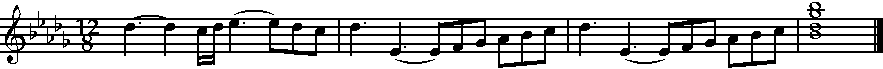
\includegraphics[width=\linewidth]{fig/mtx/ring_finale.pdf}
  \caption*{Finale of G\"otterd\"ammerung by Richard Wagner.
  Step into the mythical world of gods and heroes with our millimeter wave channel estimation simulation software.}
\end{figure}

\end{document}
\endinput
